\documentclass[12pt,a4paper,oneside]{report}
\usepackage[a4paper,left=0.86in,right=0.92in,top=0.75in,bottom=0.70in]{geometry}
\usepackage{fontspec}\setmainfont{Times New Roman}
\usepackage{setspace}\setstretch{1.15}
\usepackage{amsmath,amssymb,booktabs,tabularx,array,longtable,tikz,enumitem,caption,listings,xcolor,graphicx}
\usetikzlibrary{arrows.meta,positioning,shapes.geometric}
\usepackage[hidelinks]{hyperref}
\setcounter{tocdepth}{3}\setcounter{secnumdepth}{3}
\captionsetup{font=small,labelfont=bf}
\pagestyle{plain}
\newcommand{\notprovided}{\textit{Not provided in the available project records}}
\begin{document}
\begin{titlepage}\thispagestyle{empty}\begin{center}
\vspace*{0.35in}{\large\bfseries B.Tech. BCSE497J -- PROJECT-I\par}\vspace{0.65in}
{\Large\bfseries PHANTOM: CAUSAL ATTRIBUTION OF RUNTIME SBOM DRIFT VIA eBPF BEHAVIORAL CONTRACTS IN KUBERNETES\par}\vspace{0.55in}
Submitted in partial fulfillment of the requirements for the degree of\\[8pt]
{\Large\bfseries Bachelor of Technology}\ in Computer Science and Engineering\\[0.35in]
\begin{tabular}{p{1.8in}p{3.3in}}\toprule\textbf{Register Number}&\textbf{Student Name and Email}\\\midrule
23BDS0078&\textbf{HARSH RANJAN}\\\small\texttt{harsh.ranjan2023@vitstudent.ac.in}\\[4pt]23BDS0191&\textbf{JAI GOEL}\\\small\texttt{jai.goel2023@vitstudent.ac.in}\\\bottomrule\end{tabular}\\[0.35in]
Under the Supervision of\\[5pt]{\large\bfseries Dr. THANUJA R}\\\texttt{thanuja.r@vit.ac.in}\\Vellore Institute of Technology\\School of Computer Science and Engineering (SCOPE)
\vfill
\includegraphics[width=3.75in]{vit-logo.png}
\end{center}\end{titlepage}
\pagenumbering{roman}
\chapter*{Declaration}\addcontentsline{toc}{chapter}{Declaration}
We hereby declare that the project entitled \emph{PHANTOM: Causal Attribution of Runtime SBOM Drift via eBPF Behavioral Contracts in Kubernetes}, submitted for the award of the degree of Bachelor of Technology in Computer Science and Engineering to Vellore Institute of Technology, is a record of project work carried out under the supervision of Dr. Thanuja R. The technical statements and results in this report are limited to the source code and records identified in the report. This work has not been submitted in whole or in part for another degree or diploma.

Place: Vellore \hfill Date: October 2026\\[0.6in]
\begin{tabularx}{\textwidth}{>{\centering\arraybackslash}X >{\centering\arraybackslash}X}\hrulefill&\hrulefill\\[-2pt]Harsh Ranjan&Jai Goel\end{tabularx}
\chapter*{Certificate}\addcontentsline{toc}{chapter}{Certificate}
This is to certify that the project entitled \emph{PHANTOM: Causal Attribution of Runtime SBOM Drift via eBPF Behavioral Contracts in Kubernetes}, submitted by Harsh Ranjan and Jai Goel, School of Computer Science and Engineering, Vellore Institute of Technology, is a record of project work carried out under my supervision. This report describes the current research prototype and distinguishes implemented software from results that remain experimentally unverified.

Place: Vellore \hfill Date: \rule{1.2in}{0.4pt}\\[0.6in]
\begin{flushright}\hrulefill\\Signature of the Guide\\Dr. Thanuja R\end{flushright}
\chapter*{Acknowledgements}\addcontentsline{toc}{chapter}{Acknowledgements}
We acknowledge the academic supervision of Dr. Thanuja R and the facilities of Vellore Institute of Technology that supported this Project-I work. We also acknowledge the maintainers of the open-source projects and research tools referenced in this report. The project artifacts were reviewed to distinguish implemented components from claims that still require controlled evaluation.
\begin{flushright}Harsh Ranjan\\Jai Goel\end{flushright}
\tableofcontents\listoffigures\listoftables
\chapter*{List of Abbreviations}\addcontentsline{toc}{chapter}{List of Abbreviations}
\begin{longtable}{p{1.3in}p{4.8in}}ATE&Average Treatment Effect\\BDG&Behavioral Dependency Graph\\BIC&Bayesian Information Criterion\\CO-RE&Compile Once -- Run Everywhere\\eBPF&Extended Berkeley Packet Filter\\ECE&Expected Calibration Error\\FPR&False-Positive Rate\\IMA&Integrity Measurement Architecture\\KL&Kullback--Leibler Divergence\\PCEPS&Predictive Compromise Exposure Probability Score (unvalidated prioritization score)\\PURL&Package URL\\RCA&Root-Cause Analysis\\SBOM&Software Bill of Materials\\SCM&Structural Causal Model\end{longtable}
\chapter*{Symbols and Notations}\addcontentsline{toc}{chapter}{Symbols and Notations}
\begin{longtable}{p{1.3in}p{4.8in}}$G=(V,E)$&Typed Behavioral Dependency Graph\\$\Sigma$&Behavioral token alphabet\\$h$&Markov context\\$N$&Number of training tokens\\$K_{\max}$&Maximum candidate model order\\$D_{\mathrm{KL}}$&Conditional divergence score, in nats\\$\lambda,\Delta$&BDG decay parameter and time scale\\$q_e$&Incremental edge-evidence weight\\$S,D,X$&Candidate treatment, drift outcome, and covariates\end{longtable}
\chapter*{Abstract}\addcontentsline{toc}{chapter}{Abstract}
\begin{spacing}{1.15}
Cloud-native applications combine software components whose behavior may change after deployment. A software bill of materials (SBOM) records component inventory, while runtime monitors observe process, file, and network activity. Neither source alone establishes which component produced an event or whether a component change caused behavioral drift. This project studies PHANTOM, a research prototype connecting SBOM-facing identity and verification interfaces with eBPF runtime collection, variable-order Markov behavioral contracts, a time-decayed Behavioral Dependency Graph (BDG), a DoWhy causal-estimation pathway, an XGBoost-based PCEPS scoring path, and evidence reporting.

The repository implements contract training with Bayesian Information Criterion (BIC) order selection, Laplace-smoothed transition probabilities, and Kullback--Leibler (KL) divergence scoring. It also contains typed graph updates, a temporal causal projection, explicit \texttt{not\_identifiable} outcomes, a 16-feature PCEPS pipeline, and report-generation services. These are implementation capabilities; they have not all been validated together in a live deployment. The drift scorer does not implement a calibrated alert threshold. The temporal ordering is a modeling assumption and does not establish causation. PCEPS model and calibration outputs were not present in the supplied experiment artifacts.

The saved evaluation set contains nine records: six completed attacks across XZ-style backdoor and dependency-confusion scenarios, and three failed SolarWinds-style injections. Each completed run contains a recorded drift event. Injection-to-first-event latency has a mean of 15.74 seconds, median of 5.52 seconds, and linearly interpolated 95th percentile of 54.72 seconds. This is an event-presence result, not verified package-level detection accuracy. Event records lack resolved SBOM/PURL bindings and independent component-level ground truth. The evaluation also lacks valid benign controls and reproducible CPU, memory, and event-loss measurements. Therefore false-positive rates, causal attribution accuracy, predictive validity, and operational overhead cannot be established. This report documents the prototype, its evidence limits, and experiments needed to evaluate identity resolution, causal attribution, and risk prioritization under controlled conditions.
\end{spacing}
\noindent\textbf{Keywords:} software supply-chain security, Kubernetes, eBPF, runtime drift, SBOM, causal estimation, behavioral contracts.
\clearpage\pagenumbering{arabic}
\chapter{Introduction}
\section{Background}
Cloud-native systems combine third-party packages, container images, build systems, and deployment configuration. Supply-chain incidents such as XZ Utils and SUNBURST show that a trusted distribution path can still produce behavior that warrants investigation [1]--[4]. An SBOM describes components at a point in a build or scan [10], [11], while runtime monitors observe operating-system events and may apply rules or policies [7]--[9]. Neither alone always links an event to the package responsible or establishes causation.
\section{Motivation}
A process event can be difficult to interpret when code is loaded from multiple packages or a package changes without changing its name. An inventory does not show what a deployed component did. PHANTOM studies how identity, runtime behavior, graph evidence, and explicit uncertainty can be combined without treating an association as causal proof.
\section{Scope of the Project}
The project includes SBOM verification interfaces, eBPF event collection, image/PURL-scoped contracts, drift scoring, BDG maintenance, causal-estimation eligibility, PCEPS, and evidence reports. The saved evaluation supports only event presence and first-event latency. Component attribution, calibrated prediction, false-alarm behavior, and overhead remain unestablished.
\section{Organization}
Chapter 2 describes goals and related work; Chapter 3 technical requirements; Chapter 4 design; Chapter 5 methodology and tests; Chapter 6 demonstration pathway; Chapter 7 results and discussion; Chapter 8 conclusion; Chapter 9 references.

\chapter{Project Description and Goals}
\section{Literature Review}
Falco, Tetragon, and Tracee provide runtime events, rules, policy enforcement, or forensic capabilities depending on configuration [7]--[9]. CycloneDX and NTIA guidance address inventory and exchange [10], [11]. Syft and Cosign provide SBOM generation and signing/verification tools [20], [21], [27]. Bomfather studies build-time eBPF dependency observation and SBOM generation [29]; eBPF/IMA work studies SBOM enforcement in Linux [30]. Runtime/SBOM integration alone is therefore not PHANTOM's novelty. DoWhy is a general causal workflow [16]; applying it to runtime evidence depends on graph assumptions, treatment/outcome definitions, confounding control, and independent ground truth. Cloud incident RCA is adjacent work, but ranked explanations are not automatically intervention estimates [14], [15].
\section{Research Gap}
PHANTOM asks whether runtime observations can be mapped to trusted package identities and whether an assumption-explicit temporal causal path supports better explanations than event presence or graph ranking. Current records cannot answer this because PURL bindings and component-level labels are missing.
\section{Objectives}
\begin{enumerate}[leftmargin=*]\item Verify SBOM and image identity inputs.\item Train image/PURL-scoped behavioral contracts.\item Calculate divergence and novelty without calling them probabilities.\item Maintain a typed, time-decayed BDG.\item Estimate causal effects only under implemented eligibility checks; otherwise abstain.\item Score PCEPS only when trained artifacts are available.\item Produce evidence-based reports and evaluate without overclaiming.\end{enumerate}
\section{Problem Statement}
Given a trusted SBOM, identified image, contract, and runtime observations, record supported deviations and associate them with a component only when identity evidence supports the mapping. Causal outputs must retain assumptions and abstain when eligibility checks fail. The saved evaluation does not resolve events to PURLs or include an independent attribution oracle.
\section{Project Plan}
\begin{table}[htbp]\centering\caption{Project work status}\label{tab:plan}\begin{tabularx}{\textwidth}{p{1.1in}X X}\toprule Phase&Evidence&Status / next action\\\midrule Prototype&SBOM, eBPF, contract, graph, causal, scoring, gateway, reporting code&Implemented; selected unit paths tested\\Initial evaluation&Six completed attacks; three failed injections&Event presence and latency; repair failed injections\\Identity evaluation&Runtime identity ambiguous/unresolved&Collect independent process/container/PURL ground truth\\Control evaluation&No valid benign raw3 controls&Run matched benign workload, update, load, restart controls\\Prediction and overhead&No model evaluation or reliable resource samples&Evaluate held-out outcomes and collect telemetry\\\bottomrule\end{tabularx}\end{table}

\chapter{Technical Specification}
\section{Requirements}
\subsection{Functional Requirements}
Accept an SBOM, image digest and signature evidence; receive supported runtime events; build scoped contracts; calculate conditional KL and novelty; update a graph idempotently with decayed edges; check causal inputs and return an estimate or \texttt{not\_identifiable}; score PCEPS only with model/calibration; and report missing evidence.
\subsection{Non-Functional Requirements}
The repository uses modular services and versioned JSON contracts. It should preserve provenance, handle duplicate events, expose missing fields, and avoid assigning unresolved processes to packages. The README lists Python 3.11+, Docker Compose, Terraform/Helm, and Linux CO-RE requirements. No production availability target or overhead bound is verified.
\section{Feasibility Study}
\subsection{Technical Feasibility}
Service code and tests exist, and infrastructure definitions include AWS EKS. Raw experiment records lack complete kernel, Kubernetes, runtime, image-digest and source-commit details. The architecture is prototyped; reproducible end-to-end evaluation remains future work.
\subsection{Economic Feasibility}
No cloud invoices, instance-hour totals, licensing costs, or staff-time estimates were found. No numerical cost estimate is made. A future cost study should record compute, storage, monitoring, and cluster duration.
\subsection{Social Feasibility}
Runtime telemetry may expose process and network metadata. A deployment should minimize collected fields, restrict access, and set retention limits. No production privacy assessment is available.
\section{System Specification}
\subsection{Hardware Specification}
Host type, CPU, memory, and kernel build for raw3 runs are \notprovided. Zero-valued metric snapshots do not establish resource usage.
\subsection{Software Specification}
\begin{table}[htbp]\centering\caption{Environment facts in the repository}\label{tab:software}\begin{tabularx}{\textwidth}{p{1.6in}X}\toprule Item&Available information\\\midrule Language&Python 3.11+ README requirement; exact run version missing\\Orchestration&Docker Compose, Terraform/Helm; EKS definitions present\\Telemetry&Linux eBPF/CO-RE requirement; collector version missing\\SBOM&CycloneDX and PURL support in code\\Causal&DoWhy adapter; experiment version missing\\PCEPS&XGBoost/Platt code; trained experiment model absent\\Revision&Experiment commit not linked to runs\\\bottomrule\end{tabularx}\end{table}

\chapter{Design Approach and Details}
\section{System Architecture}
Figure~\ref{fig:arch} is a repository-based logical design, not proof that every stage ran in the experiments.
\begin{figure}[htbp]\centering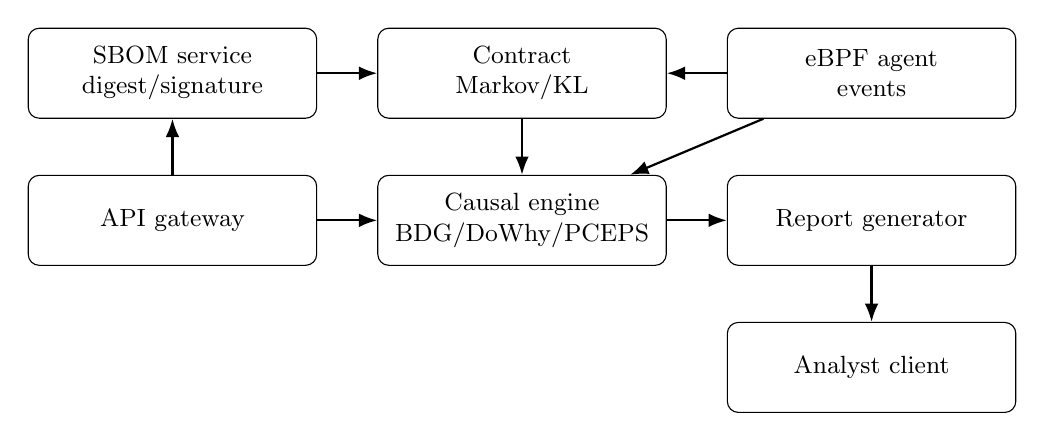
\begin{tikzpicture}[b/.style={draw,rounded corners,align=center,text width=1.35in,minimum height=.45in,font=\small},a/.style={-{Latex},thick},node distance=.28in and .3in]
\node[b](sb){SBOM service\\digest/signature};\node[b,right=of sb](ct){Contract\\Markov/KL};\node[b,right=of ct](eb){eBPF agent\\events};\node[b,below=of ct](cg){Causal engine\\BDG/DoWhy/PCEPS};\node[b,left=of cg](gw){API gateway};\node[b,right=of cg](rg){Report generator};\node[b,below=of rg](ui){Analyst client};
\draw[a](sb)--(ct);\draw[a](eb)--(ct);\draw[a](ct)--(cg);\draw[a](eb)--(cg);\draw[a](gw)--(sb);\draw[a](gw)--(cg);\draw[a](cg)--(rg);\draw[a](rg)--(ui);\end{tikzpicture}\caption{Logical service architecture from repository modules}\label{fig:arch}\end{figure}
The gateway exposes operations to the analyst client; the report generator assembles evidence. Event-to-PURL mapping is an evidence boundary: identity that cannot be resolved must remain unresolved.
\section{Design}
\subsection{Data Flow Diagram}
Figure~\ref{fig:flow} summarizes the evidence gates.
\begin{figure}[htbp]\centering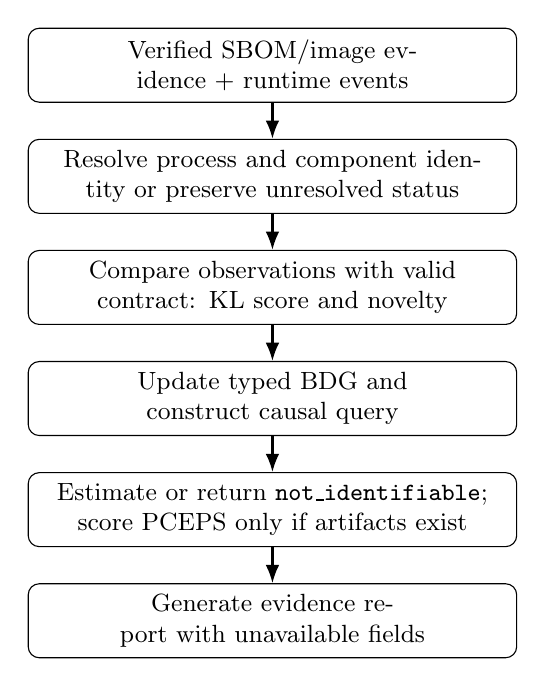
\begin{tikzpicture}[b/.style={draw,rounded corners,align=center,text width=2.35in,minimum height=.37in,font=\small},a/.style={-{Latex},thick},node distance=.18in]
\node[b](f1){Verified SBOM/image evidence + runtime events};\node[b,below=of f1](f2){Resolve process and component identity or preserve unresolved status};\node[b,below=of f2](f3){Compare observations with valid contract: KL score and novelty};\node[b,below=of f3](f4){Update typed BDG and construct causal query};\node[b,below=of f4](f5){Estimate or return \texttt{not\_identifiable}; score PCEPS only if artifacts exist};\node[b,below=of f5](f6){Generate evidence report with unavailable fields};
\draw[a](f1)--(f2);\draw[a](f2)--(f3);\draw[a](f3)--(f4);\draw[a](f4)--(f5);\draw[a](f5)--(f6);\end{tikzpicture}\caption{Data flow and evidence gates}\label{fig:flow}\end{figure}
\begin{enumerate}[leftmargin=*]\item Verify SBOM digest/signature.\item Normalize supported events and resolve runtime identity.\item Preserve unresolved identity where mapping evidence is missing.\item Compare valid event windows with a contract using KL and novelty.\item Update typed BDG evidence and temporal weights.\item Check causal eligibility; estimate or return \texttt{not\_identifiable}.\item Score PCEPS only if model artifacts exist.\item Generate a report that includes unavailable fields.\end{enumerate}
\subsection{Use Case Diagram}
The service pathway supports SBOM registration, runtime event submission, and analyst review of reports. These are code-level interactions, not a validated end-to-end user study.
\begin{figure}[htbp]\centering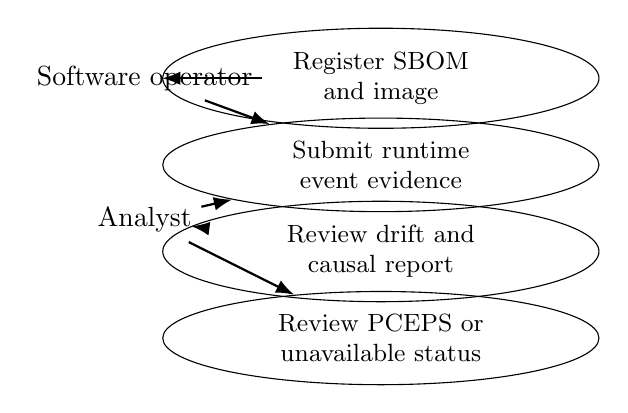
\begin{tikzpicture}[u/.style={draw,ellipse,align=center,text width=1.45in,minimum height=.42in,font=\small},a/.style={-{Latex},thick}]
\node (op) at (0,0) {Software operator};\node (an) at (0,-1.8) {Analyst};\node[u] (sb) at (3,0) {Register SBOM and image};\node[u] (ev) at (3,-1.1) {Submit runtime event evidence};\node[u] (rp) at (3,-2.2) {Review drift and causal report};\node[u] (pc) at (3,-3.3) {Review PCEPS or unavailable status};
\draw[a](op)--(sb);\draw[a](op)--(ev);\draw[a](an)--(ev);\draw[a](an)--(rp);\draw[a](an)--(pc);\end{tikzpicture}\caption{Primary project use cases}\label{fig:usecase}\end{figure}
\begin{table}[htbp]\centering\caption{Main use cases}\begin{tabularx}{\textwidth}{p{1.3in}X X}\toprule Actor&Use case&Output\\\midrule Operator&Register SBOM/image evidence&Verified/rejected artifact record\\Agent&Submit event evidence&Typed event record\\Analyst&Request report&Drift, identity and causal status\\Analyst&Review PCEPS&Score or unavailable status\\\bottomrule\end{tabularx}\end{table}
\subsection{Class Diagram}
The repository uses service/domain models rather than one monolithic class hierarchy. Conceptually, a workload/image is associated with PURLs and runtime containers/processes; events add evidence to graph relations; contracts and causal results summarize selected evidence. A process association or graph edge alone does not prove package causation.
\begin{figure}[htbp]\centering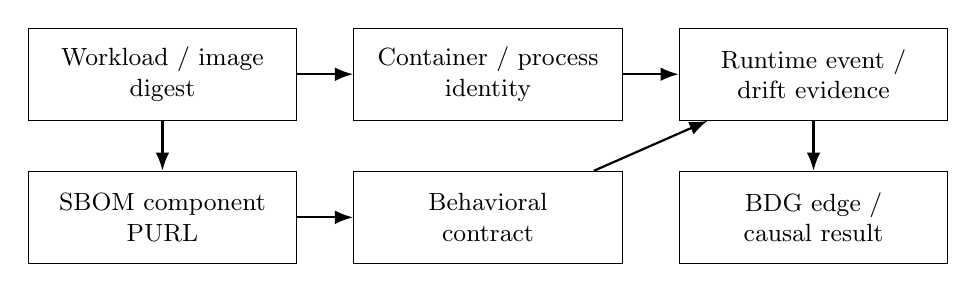
\begin{tikzpicture}[c/.style={draw,rectangle,align=center,text width=1.25in,minimum height=.46in,font=\small},a/.style={-{Latex},thick},node distance=.25in and .28in]
\node[c](w){Workload / image\\digest};\node[c,right=of w](p){Container / process\\identity};\node[c,right=of p](e){Runtime event /\\drift evidence};\node[c,below=of w](u){SBOM component\\PURL};\node[c,below=of p](k){Behavioral\\contract};\node[c,below=of e](g){BDG edge /\\causal result};\draw[a](w)--(p);\draw[a](p)--(e);\draw[a](w)--(u);\draw[a](u)--(k);\draw[a](k)--(e);\draw[a](e)--(g);\end{tikzpicture}\caption{Conceptual entity relationships}\label{fig:class}\end{figure}
\subsection{Sequence Diagram}
An analyst requests a report through the gateway. The gateway requests available graph, drift, attribution, and score records; the report generator assembles them and returns the result. If identity or scoring evidence is missing, the report should retain the unresolved or unavailable state.
\begin{figure}[htbp]\centering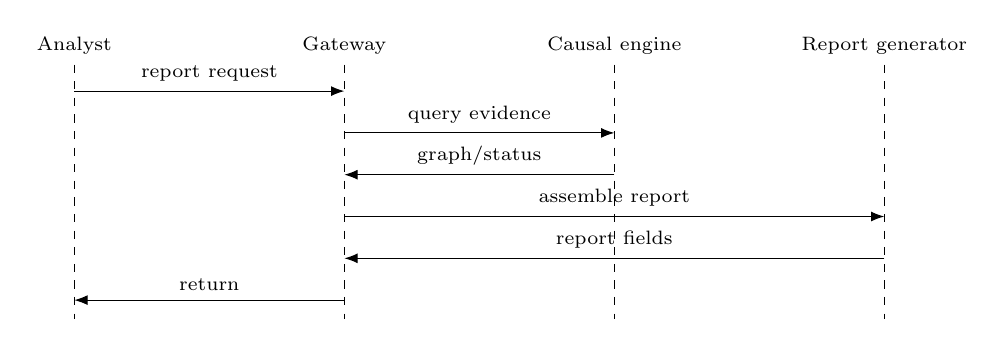
\begin{tikzpicture}[x=1in,y=.38in,>=Latex,font=\scriptsize]
\foreach \x/\n in {0/Analyst,1.35/Gateway,2.7/Causal engine,4.05/Report generator}{\node at (\x,0){\n};\draw[dashed](\x,-.25)--(\x,-3.6);}
\draw[->](0,-.6)--node[above]{report request}(1.35,-.6);\draw[->](1.35,-1.15)--node[above]{query evidence}(2.7,-1.15);\draw[->](2.7,-1.7)--node[above]{graph/status}(1.35,-1.7);\draw[->](1.35,-2.25)--node[above]{assemble report}(4.05,-2.25);\draw[->](4.05,-2.8)--node[above]{report fields}(1.35,-2.8);\draw[->](1.35,-3.35)--node[above]{return}(0,-3.35);\end{tikzpicture}\caption{Simplified report-generation sequence}\label{fig:sequence}\end{figure}

\chapter{Methodology and Testing}
\section{Module Description}
\begin{longtable}{p{1.25in}p{2.35in}p{2.3in}}\caption{Repository modules and status}\label{tab:modules}\\\toprule Module&Responsibility&Evidence status\\\midrule\endfirsthead\toprule Module&Responsibility&Evidence status\\\midrule\endhead
SBOM service&Digest, metadata and signature paths&Code exists; raw3 binding unresolved\\eBPF agent&Runtime event collection&Code exists; identity incomplete in raw3\\Contract module&Markov training/BIC/model serialization&Implemented and unit-tested\\Drift module&Conditional KL/novelty&Numeric score; no calibrated threshold\\Causal engine&BDG, projection, DoWhy&Implemented paths; no attack oracle validation\\PCEPS&16-feature XGBoost/Platt pathway&Training code; no evaluated artifacts\\API gateway&Coordinates service operations&Code and schemas present\\Report generator&Aggregates evidence&Report output does not validate cause\\\bottomrule\end{longtable}
\section{Methodology}
For candidate order $k$, the transition estimate is $\hat P_k(x\mid h)=(n_k(h,x)+1)/(n_k(h)+|\Sigma|)$. Model selection minimizes $\mathrm{BIC}(k)=-2\log L_k+q_k\log N$, where $q_k=|H_k|(|\Sigma|-1)$. Contexts are pruned when their local BIC does not improve on a retained suffix. The window score is the weighted conditional divergence
\[D_{\mathrm{KL}}=\sum_h\frac{n_h}{N}\sum_x\widehat P_{\mathrm{obs}}(x\mid h)\log\frac{\widehat P_{\mathrm{obs}}(x\mid h)}{P_{\mathrm{contract}}(x\mid h)}.\]
This is a numerical score in nats, not a calibrated anomaly probability. The scorer does not implement the proposed split-conformal alert threshold. BDG edges use $w_e(t)=\lambda^{(t-t_{prev})/\Delta}w_e(t_{prev})+q_e$. The fixed semantic causal tiers are assumptions, not proof of cause.
\section{Testing}
The available local test run reported 454 tests passed and one skipped across the core library and five service suites. These tests exercise software paths, including selected graph and causal abstention behavior. They do not estimate attack-detection accuracy, prove package attribution, or establish production performance.

\chapter{Project Demonstration}
\section{Available Demonstration Path}
The repository includes service APIs, Docker Compose and infrastructure definitions, and an analyst client. A demonstrable pathway would register SBOM/image evidence, collect events, compare a contract, inspect graph and causal status, and review a generated report. The raw runs do not establish a reproducible deployed demonstration because image digests, exact versions, and package identity links are incomplete. No verified screenshot or live demonstration transcript was found, so this report does not claim a specific observed UI session.
\section{Completed-Run Evidence}
Six completed runs contain first-event timestamps within the 120-second window. Recorded events include namespace-change or privilege-transition observations, but identity remains ambiguous or missing and PURL/SBOM fields are unresolved. These traces support event-presence and latency only.

\chapter{Result and Discussion}
\section{Experimental Setup}
The raw3 set has nine records: three XZ-style runs, three dependency-confusion runs, and three failed SolarWinds-style injections. Six completed attack phases are valid observations; failed injections are not false negatives. The exact kernel, Kubernetes and runtime versions, image digests, commit and experiment package versions are missing.
\begin{table}[htbp]\centering\caption{Run-level observed outcomes}\label{tab:runs}\begin{tabularx}{\textwidth}{Xrrrr}\toprule Family&Valid&Event+&Failed&\multicolumn{1}{c}{Evidence status}\\\midrule XZ-style&3&3&0&Identity unresolved\\Dependency confusion&3&3&0&Identity unresolved\\SolarWinds-style&0&0&3&Injection failed\\Benign control&0&--&--&No valid controls\\\bottomrule\end{tabularx}\end{table}
\section{Event Presence and Latency}
All six completed runs have a recorded drift event. The event-positive fraction is $6/6=1.000$ with two-sided 95\% Wilson score interval $[0.610,1.000]$. It is not a validated recall estimate. Latency is injection timestamp to first recorded PHANTOM event timestamp; P95 uses linear interpolation.
\begin{table}[htbp]\centering\caption{Injection-to-first-recorded-event latency}\label{tab:latency}\begin{tabular}{llr}\toprule Family&Run&Seconds\\\midrule XZ-style&1&70.332\\XZ-style&2&6.350\\XZ-style&3&4.682\\Dependency confusion&1&2.607\\Dependency confusion&2&7.876\\Dependency confusion&3&2.578\\\midrule All&Mean&15.737\\All&Median&5.516\\All&Interpolated P95&54.718\\\bottomrule\end{tabular}\end{table}
The long first XZ latency's cause is not established. The unit is a scenario run, not duplicated event rows. Without valid benign controls, true negatives, precision, recall, F1, specificity, FPR, and false alarms/hour are unavailable.
\section{Causal Attribution}
An aggregate artifact reports 1.0 attribution accuracy, but raw records contain no predicted PURLs compared with oracle target PURLs. Event identities are unresolved. Graph association and correct process identification do not prove causal correctness. The temporal projection uses fixed semantic tiers and a graph constructed partly from prescribed edges. No attribution accuracy is reported.
\section{PCEPS Results}
Training, calibration, and scoring code exists. No trained model, calibration file, scored windows, held-out labels, or reproducible performance output was found. No AUC, Brier score, calibration error, or future-compromise result is reported.
\section{Baseline Comparison}
The baseline log records Falco and Trivy setup skipped, Falco alert output missing, and Isolation Forest fit on synthetic rather than matched attack-trace frequencies. Trivy is a static vulnerability scanner. No comparative recall or superiority claim is supported.
\section{Overhead and Cost}
Saved CPU, memory and event-lag values are zero but lack raw samples and measurement provenance; they do not demonstrate zero overhead. Project cost data were not available. A future study should compare enabled/disabled monitoring under matched workloads and collect CPU, memory, application/event latency, dropped events, host versions and raw samples.
\section{Threats to Validity}
The sample covers two attack families and event presence rather than confirmed component attribution. Three injections failed, controls are absent, and package bindings are unresolved. Baseline outputs, PCEPS evaluation, overhead, and reproducibility manifest are incomplete. The causal projection depends on supplied covariates and fixed semantic ordering. These limitations prevent generalized performance or causal-correctness claims.
\section{Proposed Follow-Up Evaluation}
Freeze contracts before testing; pre-register labels; run benign package upgrades, load/configuration changes, restarts/autoscaling, both completed attacks, and repaired failed injections. Archive target PURL, image digest, process lineage, independent oracle, and PHANTOM prediction. Configure baselines for appropriate tasks on matched inputs. Split prospective PCEPS outcomes by independent run/workload. Collect resource and event-loss samples with host provenance. This is future work, not completed experimentation.

\chapter{Conclusion}
PHANTOM is an implemented prototype connecting SBOM-facing services, eBPF collection, variable-order Markov contracts, a typed time-decayed graph, causal-estimation pathways, PCEPS code, and report generation. Six completed attack runs contain recorded events and measurable injection-to-first-event latency. The evidence does not establish component-level causal attribution, calibrated prediction, benign false-positive behavior, baseline performance, or overhead. A controlled follow-up with resolved identity, ground truth, controls, matched baselines and a reproducibility manifest is required before stronger claims are made.

\renewcommand{\bibname}{References}
\begin{thebibliography}{99}
\addcontentsline{toc}{chapter}{References}
\bibitem{r1} CISA, ``Reported Supply Chain Compromise Affecting XZ Utils Data Compression Library, CVE-2024-3094,'' Alert AA24-089A, Mar. 29, 2024.
\bibitem{r2} A. Freund, ``Backdoor in upstream xz/liblzma leading to ssh server compromise,'' oss-security, Mar. 29, 2024. Available: \url{https://www.openwall.com/lists/oss-security/2024/03/29/4}
\bibitem{r3} CISA, ``Advanced Persistent Threat Compromise of Government Agencies, Critical Infrastructure, and Private Sector Organizations,'' Alert AA20-352A, Dec. 2020. Available: \url{https://www.cisa.gov/news-events/cybersecurity-advisories/aa20-352a}
\bibitem{r4} FireEye, ``Highly Evasive Attacker Leverages SolarWinds Supply Chain to Compromise Multiple Global Victims With SUNBURST Backdoor,'' Dec. 2020.
\bibitem{r5} Apache Software Foundation, ``Apache Log4j Security Vulnerabilities: CVE-2021-44228,'' 2021. Available: \url{https://logging.apache.org/log4j/2.x/security.html}
\bibitem{r6} NIST, ``CVE-2021-44228 Detail,'' NVD, 2021. Available: \url{https://nvd.nist.gov/vuln/detail/CVE-2021-44228}
\bibitem{r7} Sysdig, ``Falco: Cloud Native Runtime Security,'' project documentation. Available: \url{https://falco.org/docs/}
\bibitem{r8} Isovalent, ``Tetragon: eBPF-Based Security Observability and Runtime Enforcement,'' 2023. Available: \url{https://tetragon.io/}
\bibitem{r9} Aqua Security, ``Tracee: Linux Runtime Security and Forensics Using eBPF,'' project documentation. Available: \url{https://github.com/aquasecurity/tracee}
\bibitem{r10} OWASP, ``CycloneDX Specification, Version 1.4,'' 2022. Available: \url{https://cyclonedx.org/specification/archive/}
\bibitem{r11} U.S. Department of Commerce, ``The Minimum Elements for a Software Bill of Materials,'' NTIA, 2021. Available: \url{https://www.ntia.gov/report/2021/minimum-elements-software-bill-materials-sbom}
\bibitem{r12} Anchore, ``Anchore Enterprise: SBOM-Powered Software Supply Chain Security,'' product documentation. Available: \url{https://anchore.com/enterprise/}
\bibitem{r13} Ox Security, ``Software Supply Chain Security Platform,'' product documentation. Available: \url{https://ox.security/}
\bibitem{r14} Y. Chen et al., ``Automatic Root Cause Analysis via Large Language Models for Cloud Incidents,'' in Proc. EuroSys, 2024, pp. 674--688.
\bibitem{r15} J. Pearl, \emph{Causality: Models, Reasoning, and Inference}, 2nd ed. Cambridge University Press, 2009.
\bibitem{r16} A. Sharma and E. Kiciman, ``DoWhy: An End-to-End Library for Causal Inference,'' arXiv:2011.04216, 2020. Available: \url{https://arxiv.org/abs/2011.04216}
\bibitem{r17} Google, ``Online Boutique: Cloud-Native Microservices Demo.'' Available: \url{https://github.com/GoogleCloudPlatform/microservices-demo}
\bibitem{r18} DARPA, ``Transparent Computing Program: Data and Resources.'' Available: \url{https://www.darpa.mil/research/programs/transparent-computing}
\bibitem{r19} AccuKnox, ``KubeArmor: Container-Aware AppArmor, SELinux, and BPF Security.'' Available: \url{https://kubearmor.io/}
\bibitem{r20} Anchore, ``Syft: Generate a Software Bill of Materials from Container Images and Filesystems.'' Available: \url{https://github.com/anchore/syft}
\bibitem{r21} Sigstore, ``Cosign: Container Signing, Verification, and Storage.'' Available: \url{https://docs.sigstore.dev/cosign/}
\bibitem{r22} eBPF Foundation, ``What is eBPF?'' Available: \url{https://ebpf.io/what-is-ebpf/}
\bibitem{r23} A. A. Hagberg, D. A. Schult, and P. J. Swart, ``Exploring network structure, dynamics, and function using NetworkX,'' Proc. SciPy, 2008, pp. 11--15.
\bibitem{r24} T. Chen and C. Guestrin, ``XGBoost: A scalable tree boosting system,'' Proc. ACM SIGKDD, 2016, pp. 785--794.
\bibitem{r25} J. Platt, ``Probabilistic outputs for support vector machines and comparisons to regularized likelihood methods,'' in \emph{Advances in Large Margin Classifiers}, 1999, pp. 61--74.
\bibitem{r26} Package-URL Working Group, ``Package URL Specification.'' Available: \url{https://github.com/package-url/purl-spec}
\bibitem{r27} Sigstore, ``Cosign Documentation: Signing Containers.'' Available: \url{https://docs.sigstore.dev/cosign/signing/signing_containers/}
\bibitem{r28} Linux Foundation, ``libbpf: BPF CO-RE Reference Guide.'' Available: \url{https://github.com/libbpf/libbpf}
\bibitem{r29} N. Srinivasan, N. Naveen, and N. Naveen, ``Bomfather: An eBPF-based Kernel-level Monitoring Framework for Accurate Identification of Unknown, Unused, and Dynamically Loaded Dependencies in Modern Software Supply Chains,'' arXiv:2503.02097, 2025. Available: \url{https://arxiv.org/abs/2503.02097}
\bibitem{r30} A. Crawford, E. Yakubovich, and R. Szumski, ``Enforcing SBOMs through the Linux kernel with eBPF and IMA,'' Proc. ACM SCORED, 2023, pp. 77--78, doi: 10.1145/3605770.3625206.
\end{thebibliography}
\appendix
\chapter{Algorithm and Reproducibility Checklist}
\section{Evidence-Gated Processing}
\begin{lstlisting}[basicstyle=\ttfamily\small,breaklines=true,frame=single]
verify SBOM digest and signature; reject invalid artifact
normalize supported events; resolve runtime identity
if evidence supports component PURL: associate event
else: preserve unresolved identity
if valid contract exists: compute KL and novelty
else: mark contract comparison unavailable
update typed BDG; ignore duplicate UUID; decay edge weights
if causal eligibility checks pass: estimate and refute with DoWhy
else: return not_identifiable with diagnostic
if PCEPS model and calibration exist: compute bounded score
else: mark PCEPS unavailable
generate report from available evidence
\end{lstlisting}
\section{Reproducibility Checklist}
Record the following fields for each run:
\begin{itemize}[leftmargin=*]
\item Host type, operating system, CPU, memory, and kernel version.
\item Kubernetes and container runtime versions; collector, Python, and DoWhy versions.
\item Experiment commit, image and SBOM digests, and contract interval and settings.
\item Target PURL, independent labels, attack and control versions, and baseline configurations.
\item Raw outputs, PCEPS model and calibration digests, timestamps, event loss, resource samples, and cost records.
\end{itemize}
The current raw3 records lack several of these fields.
\end{document}